\documentclass{article}
\usepackage{fullpage}
\usepackage{booktabs}
\usepackage{amsmath}
\usepackage{amssymb}
\usepackage[noend]{algorithmic}
\usepackage[nothing]{algorithm}
\usepackage{tikz}
\usepackage{latexsym}
\usepackage{float}
\usepackage{hyperref}
\usetikzlibrary{arrows,automata}
\providecommand{\e}[1]{\ensuremath{\times 10^{#1}}}
\renewcommand{\thealgorithm}{}
\renewcommand*{\thefootnote}{[\arabic{footnote}]}
\title{CS 544: Computer Networks \\ Midterm}
\author{Dustin Ingram}
\begin{document}
\maketitle
\section{Reference Model Layers}
\subsection{TCP/IP}
Layers in order from highest to lowest:
\begin{itemize}
\item Application Layer
\begin{itemize}
\item Transport Layer Security Sublayer
\end{itemize}
\item Transport Layer
\item Internet Layer
\item Link Layer
\item Physical Layer
\end{itemize}
\subsection{OSI}
Layers in order from highest to lowest:
\begin{itemize}
\item Application Layer: This is the application interface, or API. This is how
the network protocol communicates with an application.
\item Presentation Layer: This is the layer which handles the``representation''
of the data, encryption and decryption, etc.
\item Session Layer: This is the ``users'' of a network, 
\item Transport Layer: This is the layer which provides reliable, end-to-end
transportation of pieces of data.
\item Network Layer: This is the layer that handles routing and congestion
control for individual packets. 
\item Data Link Layer: Physical link and addressing specifications, handles
sharing of a physical link.
\begin{itemize}
\item LLC Sublayer: Protocol multiplexing
\item MAC Sublayer: Media Access Control (addressing for link sharing) 
\end{itemize}
\item Physical Layer: Bit transmission. 
\end{itemize}
\subsection{ATM}
Layers in order from highest to lowest:
\begin{itemize}
\item ATM Adaption Layer
\begin{itemize}
\item Convergence Sublayer
\item Segmentation and Reassembly Sublayer
\end{itemize}
\item ATM Layer
\item Physical Layer
\begin{itemize}
\item Transmission Convergence Sublayer
\item Physical Medium Dependent Sublayer
\end{itemize}
\item User \& Management Planes 
\end{itemize}
\section{Network Protocols \& DFAs}
\subsection{How Protocols use DFAs}
Protocols use DFAs to determine state. A DFA describes every possible state the
protocol may be in, and what must occur to transition from one state to another,
typically messages sent or received or events which happen in or to the
protocol. Together, the states and transitions define the protocol, the messages
and events it can receive and respond to, and it's overall operation.

\subsection{Why DFAs have to be Deterministic}
A deterministic finite automata guarantees that when in one state, and a
transition event or message occurs, the protocol \emph{must} and \emph{will}
transition to the same subsequent state, every time.

\subsection{Updates DFA}
        \begin{figure}[!h]
            \centering
            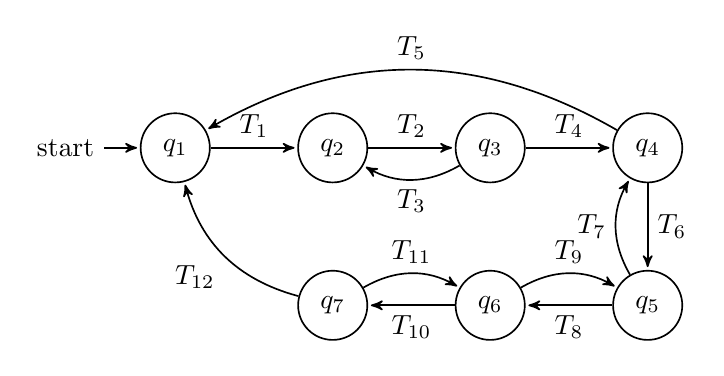
\begin{tikzpicture}[->,>=stealth',shorten >=1pt,auto,node distance=2.8cm,semithick]
              \node[state, initial]     (q1) at (0,0)  {$q_{1}$};
              \node[state]     (q2) at (2,0)  {$q_{2}$};
              \node[state]     (q3) at (4,0) {$q_{3}$};
              \node[state]     (q4) at (6,0) {$q_{4}$};
              \node[state]     (q5) at (6,-2) {$q_{5}$};
              \node[state]     (q6) at (4,-2) {$q_{6}$};
              \node[state]     (q7) at (2,-2) {$q_{7}$};

              \path (q1) edge node {$T_{1}$} (q2)
                    (q2) edge node {$T_{2}$} (q3)
                    (q3) edge[bend left] node {$T_{3}$} (q2)
                    (q3) edge node {$T_{4}$} (q4)
                    (q4) edge[bend right, above] node {$T_{5}$} (q1)
                    (q4) edge node {$T_{6}$} (q5)
                    (q5) edge[bend left] node {$T_{7}$} (q4)
                    (q5) edge node {$T_{8}$} (q6)
                    (q6) edge node {$T_{10}$} (q7)
                    (q6) edge[bend left] node {$T_{9}$} (q5)
                    (q7) edge[bend left] node {$T_{11}$} (q6)
                    (q7) edge[bend left] node {$T_{12}$} (q1)
                ;
            \end{tikzpicture}
        \end{figure}
\begin{itemize}
    \item $q_{1}$ -- Waiting for update process to begin 
    \item $q_{2}$ -- Update process is active 
    \item $q_{3}$ -- Authenticating with remote server
    \item $q_{4}$ -- Checking for updates 
    \item $q_{5}$ -- Downloading Update 
    \item $q_{6}$ -- Hashing Update 
    \item $q_{7}$ -- Installing Update 
 
\end{itemize}
\begin{itemize}
    \item $T_{1}$ -- Time since last update times out 
    \item $T_{2}$ -- Authenticate using a security mechanism 
    \item $T_{3}$ -- Authentication failed 
    \item $T_{4}$ -- Authentication successful 
    \item $T_{5}$ -- No new updates
    \item $T_{6}$ -- New updates
    \item $T_{7}$ -- Download fails 
    \item $T_{8}$ -- Download succeeds 
    \item $T_{9}$ -- Hash fails 
    \item $T_{10}$ -- Hash succeeds 
    \item $T_{11}$ -- Install fails 
    \item $T_{12}$ -- Install succeeds
\end{itemize}
\subsection{Security}
Security affects the states in the DFA of a protocol in that it adds additional states. In the example of the update protocol above, authentication is somewhat abstracted out, but there is still a state which represents it. Hashing can also be considered a security mechanism, to make sure the data is valid before installing.  

\section{Sliding Window Protocol}

\subsection{Pieces of the SWP}
\begin{itemize}
\item Sequence Numbers -- provide an ordering of messages
\item Acknowledgements
\item Positive -- acknowledge the receipt of a message or multiple message
\item Negative -- acknowledge a missing message
\item Next to receive -- acknowledge messages to a point, and indicate what is expected next
\item Windows ‐- size is necessary to keep the messages relevant to the current frame
\item Pipelining/Piggybacking -- multiple messages at once
\item Checksums -- verifying messages via checksums
\end{itemize}
\subsection{Video Protocol}
Here, the sliding window protocol would not be the same. In the case of the streaming live video, there is a definite window (some amount of time ahead of what is currently being seen) that the protocol should focus message delivery on. It would not be necessary to work on delivering packets that are no longer needed to be viewed. However, in the case of storing the data to a local disk, every piece of data being transferred is relevant and important, regardless of the window size.

A peer-to-peer distributed protocol like BitTorrent would have almost no use for a sliding window protocol with regards to the original data ordering, as it is asynchronous and distributed, thus it is accepting packets completely out of order from multiple clients. It too would want to maximize file integrity.

\section{Network Layers}
The problem of networking is broken into layers so that different aspects of the network stack can treat each other as black boxes, and simply pass the necessary data between them. This concentrates similar functions together, and allows us to mix-and-match layers as they will interoperate well, creating a ``building block'' approach where one layer stacks nicely (communicates well with) another layer.

Sublayers further separate related functions, but are grouped within a common layer. 
\subsection{Transport Layer}
Sublayers of the transport layer:
\begin{itemize}
\item End-to-End connections -- Data transfer, connection-oriented streams 
\item Quality of Service -- Reliable transfer, Error detection, Congestion and Flow Control
\end{itemize}

\section{Common Themes}
Some common themes repeat themselves through multiple different protocols. This is because there are a number of things which most protocols need to operate. For example:
\begin{itemize}
\item Addressing -- A protocol must know how to address it's recipient
\item Ordered Delivery -- Out-of-ordered delivery is generally not useful, especially when working with large amounts of ordered data
\item Segmentation \& Reassembly -- Dividing data based on the limits of a protocol's message size
\item Error Detection \& Correction -- In lossy networking environments, or in situations where traffic may be manipulated, this is essential
\item Flow Control -- Ensures that clients with differing connection speeds can still communicate without being overwhelmed.

\end{itemize}
\section{Common Themes In TCP}
Here are those same themes, as they relate to one specific protocol, TCP:
\begin{itemize}
\item Addressing -- TCP uses an IP address and a port, which are encapsulated into the header of the IP packet
\item Ordered Delivery -- TCP ensures an in-order delivery by using sequence numbers
\item Segmentation \& Reassembly -- TCP splits the message into segments, which are re-assembled and ordered upon receipt 
\item Error Detection \& Correction -- TCP uses sequence numbers, a checksum and ACKs to discover and compensate for missing or corrupted packets
\item Flow Control -- TCP uses a SWP to reduce congestion and assure that the intended recipient can process the messages successfully
\end{itemize}

\section{Extensibility}
Extensibility is an important part of a good protocol because it allows the protocol to evolve over time without the need for modification of the core protocol. It also allows protocols to be fixed, or support new feature sets that were not originally considered or beyond the scope of the original protocol. Extensibility also allows implementors to potentially customize or tweak the protocol to their desire, and therefore allows for reuse.

\subsection{XMPP and Extensibility}
XMPP is inherently extendable -- after all, it's in the name. Within the XMPP
protocol lies a number of XMPP Extension Protocols, otherwise known as XEPs,
which provide additional functionality across a wide range of applications on
top of the core protocol. For example, XEP-0045 defines an extension for
multi-user chat, which builds upon this RFC in the same way that this RFC builds
upon other standards.

These XEPs can essentially modify the message body, the addressing of the messages, etc. The original specification provides enough flexibility with the base protocol that nearly any extension can be added without core modification. 

\subsection{FTP and Extensibility}
An extension to the FTP protocol requires an addition of a command or command set -- for example, FTPS (FTP Secure) requires an additional `auth' command.
\end{document}
